\documentclass{article}\usepackage[]{graphicx}\usepackage[]{color}
%% maxwidth is the original width if it is less than linewidth
%% otherwise use linewidth (to make sure the graphics do not exceed the margin)
\makeatletter
\def\maxwidth{ %
  \ifdim\Gin@nat@width>\linewidth
    \linewidth
  \else
    \Gin@nat@width
  \fi
}
\makeatother

\definecolor{fgcolor}{rgb}{0.345, 0.345, 0.345}
\newcommand{\hlnum}[1]{\textcolor[rgb]{0.686,0.059,0.569}{#1}}%
\newcommand{\hlstr}[1]{\textcolor[rgb]{0.192,0.494,0.8}{#1}}%
\newcommand{\hlcom}[1]{\textcolor[rgb]{0.678,0.584,0.686}{\textit{#1}}}%
\newcommand{\hlopt}[1]{\textcolor[rgb]{0,0,0}{#1}}%
\newcommand{\hlstd}[1]{\textcolor[rgb]{0.345,0.345,0.345}{#1}}%
\newcommand{\hlkwa}[1]{\textcolor[rgb]{0.161,0.373,0.58}{\textbf{#1}}}%
\newcommand{\hlkwb}[1]{\textcolor[rgb]{0.69,0.353,0.396}{#1}}%
\newcommand{\hlkwc}[1]{\textcolor[rgb]{0.333,0.667,0.333}{#1}}%
\newcommand{\hlkwd}[1]{\textcolor[rgb]{0.737,0.353,0.396}{\textbf{#1}}}%

\usepackage{framed}
\makeatletter
\newenvironment{kframe}{%
 \def\at@end@of@kframe{}%
 \ifinner\ifhmode%
  \def\at@end@of@kframe{\end{minipage}}%
  \begin{minipage}{\columnwidth}%
 \fi\fi%
 \def\FrameCommand##1{\hskip\@totalleftmargin \hskip-\fboxsep
 \colorbox{shadecolor}{##1}\hskip-\fboxsep
     % There is no \\@totalrightmargin, so:
     \hskip-\linewidth \hskip-\@totalleftmargin \hskip\columnwidth}%
 \MakeFramed {\advance\hsize-\width
   \@totalleftmargin\z@ \linewidth\hsize
   \@setminipage}}%
 {\par\unskip\endMakeFramed%
 \at@end@of@kframe}
\makeatother

\definecolor{shadecolor}{rgb}{.97, .97, .97}
\definecolor{messagecolor}{rgb}{0, 0, 0}
\definecolor{warningcolor}{rgb}{1, 0, 1}
\definecolor{errorcolor}{rgb}{1, 0, 0}
\newenvironment{knitrout}{}{} % an empty environment to be redefined in TeX

\usepackage{alltt}

\usepackage{tikz}
\IfFileExists{upquote.sty}{\usepackage{upquote}}{}
\begin{document}




\begin{knitrout}\footnotesize
\definecolor{shadecolor}{rgb}{0.969, 0.969, 0.969}\color{fgcolor}\begin{kframe}
\begin{alltt}
\hlkwd{library}\hlstd{(ggplot2)}
\hlkwd{library}\hlstd{(ggpmisc)}
\end{alltt}
\end{kframe}
\end{knitrout}

\begin{knitrout}\footnotesize
\definecolor{shadecolor}{rgb}{0.969, 0.969, 0.969}\color{fgcolor}\begin{kframe}
\begin{alltt}
\hlcom{# generate artificial data}
\hlkwd{set.seed}\hlstd{(}\hlnum{4321}\hlstd{)}
\hlstd{x} \hlkwb{<-} \hlnum{1}\hlopt{:}\hlnum{100}
\hlstd{y} \hlkwb{<-} \hlstd{(x} \hlopt{+} \hlstd{x}\hlopt{^}\hlnum{2} \hlopt{+} \hlstd{x}\hlopt{^}\hlnum{3}\hlstd{)} \hlopt{+} \hlkwd{rnorm}\hlstd{(}\hlkwd{length}\hlstd{(x),} \hlkwc{mean} \hlstd{=} \hlnum{0}\hlstd{,} \hlkwc{sd} \hlstd{=} \hlkwd{mean}\hlstd{(x}\hlopt{^}\hlnum{3}\hlstd{)} \hlopt{/} \hlnum{4}\hlstd{)}
\hlstd{my.data} \hlkwb{<-} \hlkwd{data.frame}\hlstd{(x,}
                      \hlstd{y,}
                      \hlkwc{group} \hlstd{=} \hlkwd{c}\hlstd{(}\hlstr{"A"}\hlstd{,} \hlstr{"B"}\hlstd{),}
                      \hlkwc{y2} \hlstd{= y} \hlopt{*} \hlkwd{c}\hlstd{(}\hlnum{0.5}\hlstd{,}\hlnum{2}\hlstd{),}
                      \hlkwc{block} \hlstd{=} \hlkwd{c}\hlstd{(}\hlstr{"a"}\hlstd{,} \hlstr{"a"}\hlstd{,} \hlstr{"b"}\hlstd{,} \hlstr{"b"}\hlstd{))}

\hlkwd{str}\hlstd{(my.data)}
\end{alltt}
\begin{verbatim}
## 'data.frame':	100 obs. of  5 variables:
##  $ x    : int  1 2 3 4 5 6 7 8 9 10 ...
##  $ y    : num  -27205 -14243 45791 53731 -8029 ...
##  $ group: Factor w/ 2 levels "A","B": 1 2 1 2 1 2 1 2 1 2 ...
##  $ y2   : num  -13603 -28485 22895 107463 -4014 ...
##  $ block: Factor w/ 2 levels "a","b": 1 1 2 2 1 1 2 2 1 1 ...
\end{verbatim}
\end{kframe}
\end{knitrout}

\begin{knitrout}\footnotesize
\definecolor{shadecolor}{rgb}{0.969, 0.969, 0.969}\color{fgcolor}\begin{kframe}
\begin{alltt}
\hlcom{# plot}
\hlkwd{ggplot}\hlstd{(}\hlkwc{data} \hlstd{= my.data,} \hlkwc{mapping}\hlstd{=}\hlkwd{aes}\hlstd{(}\hlkwc{x} \hlstd{= x,} \hlkwc{y} \hlstd{= y2,} \hlkwc{colour} \hlstd{= group))} \hlopt{+}
  \hlkwd{geom_point}\hlstd{()} \hlopt{+}
  \hlkwd{geom_smooth}\hlstd{(}\hlkwc{method} \hlstd{=} \hlstr{"lm"}\hlstd{,} \hlkwc{se} \hlstd{=}  \hlnum{FALSE}\hlstd{,}
              \hlkwc{formula} \hlstd{= y} \hlopt{~} \hlkwd{poly}\hlstd{(}\hlkwc{x}\hlstd{=x,} \hlkwc{degree} \hlstd{=} \hlnum{2}\hlstd{,} \hlkwc{raw} \hlstd{=} \hlnum{TRUE}\hlstd{))} \hlopt{+}
  \hlkwd{stat_poly_eq}\hlstd{(}
    \hlkwc{mapping}     \hlstd{=} \hlkwd{aes}\hlstd{(}\hlkwc{label} \hlstd{=} \hlkwd{paste}\hlstd{(}\hlstr{"$"}\hlstd{, ..eq.label..,} \hlstr{"$\textbackslash{}\textbackslash{} \textbackslash{}\textbackslash{} \textbackslash{}\textbackslash{} $"}\hlstd{,}
                                    \hlstd{..rr.label..,} \hlstr{"$"}\hlstd{,} \hlkwc{sep} \hlstd{=} \hlstr{""}\hlstd{))}
    \hlstd{,} \hlkwc{geom}        \hlstd{=} \hlstr{"text"}
    \hlstd{,} \hlkwc{formula}     \hlstd{= y} \hlopt{~} \hlkwd{poly}\hlstd{(x,} \hlnum{2}\hlstd{,} \hlkwc{raw} \hlstd{=} \hlnum{TRUE}\hlstd{)}
    \hlstd{,} \hlkwc{eq.with.lhs} \hlstd{=} \hlstr{"\textbackslash{}\textbackslash{}hat\{Y\} = "}
    \hlstd{,} \hlkwc{output.type} \hlstd{=} \hlstr{"LaTeX"}
   \hlstd{)} \hlopt{+}
  \hlkwd{theme_bw}\hlstd{()}
\end{alltt}
\begin{verbatim}
## [1] "\\hat{Y} = 13900 - 2230 x + 67.5 x^2"
## [1] "\\hat{Y} = 169000 - 14400 x + 327 x^2"
\end{verbatim}
\end{kframe}

{\centering 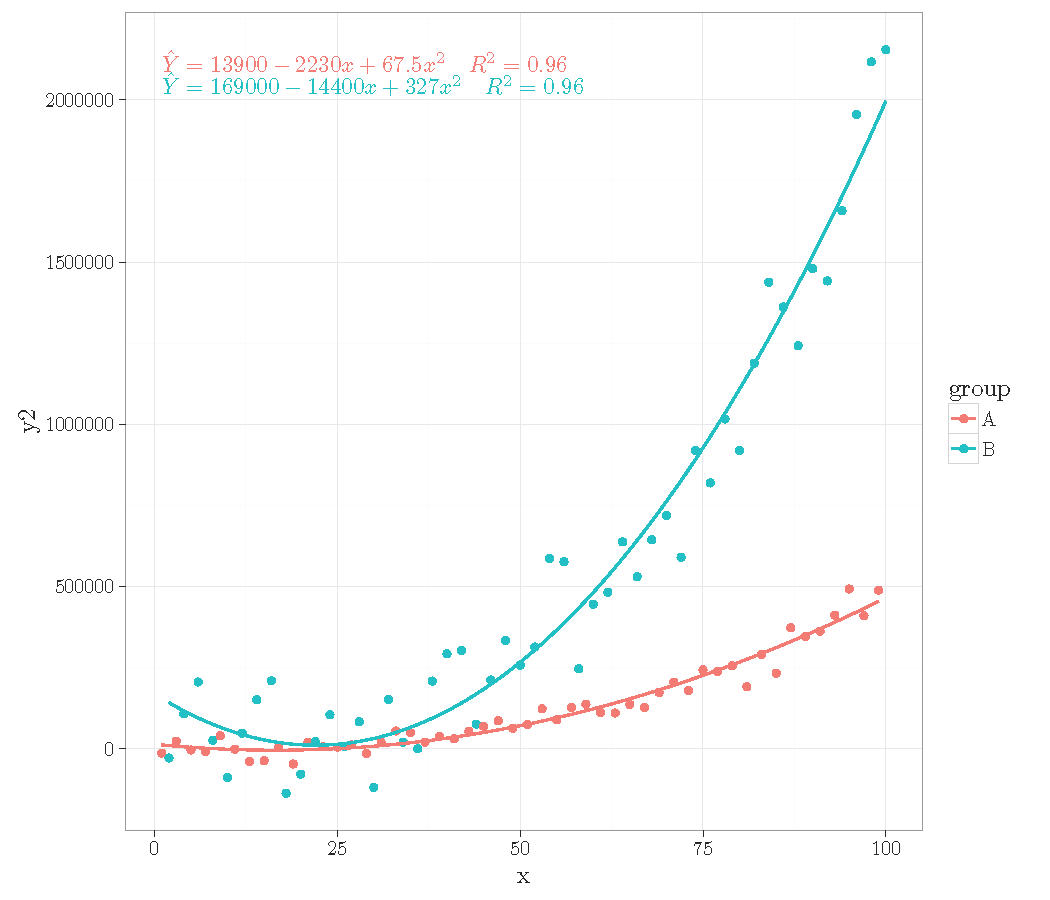
\includegraphics[width=\maxwidth]{figure/pos-unnamed-chunk-3-1} 

}



\end{knitrout}

\end{document}

